\section{TESLA based on GstLAL}
\subsection{Connecting to a LIGO Data Grid}
\subsubsection{How to Add a SSH Key}

When you are using TESLA, it's very convenient to connect to LIGO Data Grid.

This guide follows \href{https://computing.docs.ligo.org/guide/computing-centres/ldg/}{the LIGO Computing Guide}.

Because we are KAGRA member, please enter \href{https://registry.gw-astronomy.org/}{GW-Astronomy Registry}.\footnote{The link for offline(paper-book) users: https://registry.gw-astronomy.org/}

Click 'Services' on the left and click 'Click to Request' of 'LDG Account Request' among the main items.

\begin{figure}[h]
\centering
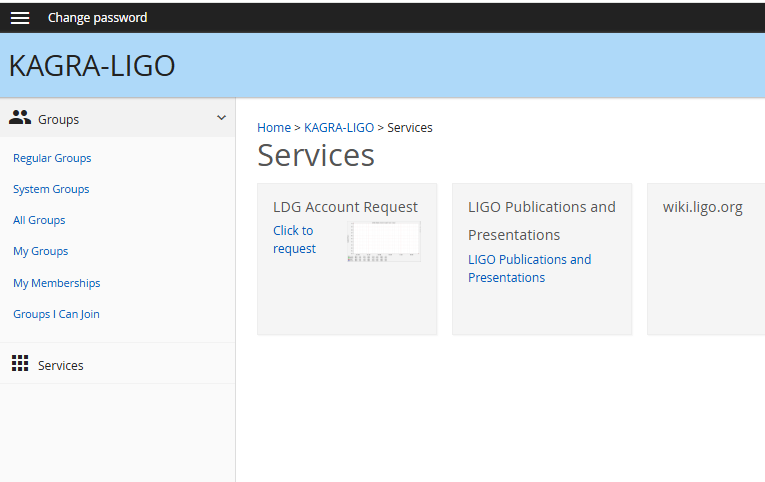
\includegraphics[width=0.6\textwidth]{figs/profile.png}
\caption{Add a SSH key}
\end{figure}

Affiliation has to be selected as 'Student', and the purpose of the current study has to be roughly written in the Justification. And click 'SUBMIT'.

Read the authorize form and aggree, and go to the next step.

And then click 'Authenticators'. Then you can see 'Add LDG SSH key' page, and in that page, you can add your SSH PUBLIC key. If you don't have an SSH key, see section \ref{SSH}.

\subsubsection{Login to the LIGO Data Grid}

If you uploaded the SSH key, you can enter to the LIGO Data Grid(the remote computer). It may take some time for the SSH key to be uploaded and logged in.

You can see the login hosts of \href{https://computing.docs.ligo.org/guide/computing-centres/hawk/}{Hawk}, \href{https://computing.docs.ligo.org/guide/computing-centres/cit/}{Caltech}, \href{https://computing.docs.ligo.org/guide/computing-centres/iucaa/}{IUCAA}, \href{https://computing.docs.ligo.org/guide/computing-centres/lho/}{LIGO-Hanford}, \href{https://computing.docs.ligo.org/guide/computing-centres/llo/}{LIGO-Livingston}, \href{https://computing.docs.ligo.org/guide/computing-centres/nemo/}{Nemo(UWM)} or \href{https://computing.docs.ligo.org/guide/computing-centres/psu/}{Gwave(PSU)}. I usually login to Caltech host.

\begin{verbatim}
    $ ssh seonjun.kwon@ldas-pcdev2.ligo.caltech.edu
\end{verbatim}

\subsection{Install the TESLA}

You can use GstLAL in LIGO Grid, or another supercomputer(for example, RESCEUBBC).

This guide was written with the help of Dr. Alvin Li.

\subsubsection{Use TESLA in the LIGO Grid}

Login to LIGO Grid and make a directory.

\begin{verbatim}
    $ mkdir Lensing
    $ cd Lensing
\end{verbatim}

There is a package in Dr. Alvin Li's directory that he has organized for download in batches.

\textbf{Use the Environment Directly: Recommended}

I recommend to use Dr Alvin Li's virtual environment directly, because Dr. Alvin Li can upgrade the elements of the TESLA environment, and in that case, it's very annoying to copy the new environment (upgrade the environment).

Set the nickname of the directory. For example, 'lensingenv'.

Vim into the '.bashrc' file.

\begin{verbatim}
    $ vi ~/.bashrc
\end{verbatim}

Add a phrase as below,

\begin{verbatim}
    export lensingenv=home/alvin.li/.conda/envs/tesla_o4a_analysis_240331/
\end{verbatim}

And reload the bashrc file.

\begin{verbatim}
    $ source ~/.bashrc
\end{verbatim}

The setup is over, so you don't have to modify or reload the '.bashrc' file as above from next time, even if you start the session anew.

You can load a virtual environment right away.

\begin{verbatim}
    $ conda activate $lensingenv
\end{verbatim}

\textbf{Install the Environment: NOT Recommended}

Let's create a Conda virtual environment by copying it.

\begin{verbatim}
    $ conda create --name testlensing --clone \
        /home/alvin.li/.conda/envs/tesla_o4a_analysis_240331
\end{verbatim}

This is the end of the installation.

The name of the package should not overlap. For example, if you set it to igwn-py39, you get an error that the name overlaps.

\subsubsection{Use TESLA in Another Supercomputer}

Basically, you can follow \href{https://git.ligo.org/alvin.li/tesla/-/tree/o4a_version_1.0}{Dr. Alvin Li's TESLA guide} in its entirety. It has been approved that it is okay to copy-paste all of this guide, and parts that are not in the guide will also be described here.

\textbf{SSH Login}

You need permission to connect to LIGO GIT on that supercomputer. Let's create an SSH key in the Ed25519 format from the home directory.

\begin{verbatim}
    $ ssh-keygen -t ed25519
    $ cd .ssh
    $ vi id_ed25519.pub
\end{verbatim}

Go to the \href{https://git.ligo.org/-/user_settings/ssh_keys}{SSH key page} of the User Settings page of the LIGO GIT.(You need to login to the LIGO GIT.) And click 'Add new key' button.

Copy and paste the entire contents of your 'ed\_25519.pub' file into the 'key' column. And click 'Add key'. Then you will get permission to clone the package files.

\textbf{Conda Environment}

You will need to first create a working python3 conda environment. We have a suggested conda YAML file included in this git repo tesla\_conda.yaml. Download the conda yml file via

\begin{verbatim}
    $ mkdir lensingenv
    $ cd lensingenv
    $ git archive --remote=git@git.ligo.org:alvin.li/tesla.git
        o4a_version_1.0 tesla_conda.yaml | tar -x
\end{verbatim}

Vim into tesla\_conda.yaml. In the last line, modify name: igwn-py39 to the name of the conda environment you want, for example, tesla\_o4a\_py39\_231228.

Of course, you don't need to vim that file and change the environment name, if you don't have 'igwn-py39' already.

Enter below.

\begin{verbatim}
    $ conda env create --file tesla_conda.yaml
\end{verbatim}

Activate the environment.

\begin{verbatim}
    $ conda activate igwn-py39
\end{verbatim}

\textbf{python-ligo-lw}

From now on, proceed with the igwn-py39 virtual environment in operation. (If not activate, enter below.)

\begin{verbatim}
    $ conda activate igwn-py39
\end{verbatim}

Because the cluster's ligolw is not up to date (especially for ligolw\_sqlite), we will need to install our own version of ligolw. To do so, first go to the conda environment directory that you have built.

For example, you can check the directory with

\begin{verbatim}
    $ vi ~/.conda/environments.txt
\end{verbatim}

And go into the directory that says igwn-py39 is in this text file. For example, (The directory may vary depending on the person or environment.)

\begin{verbatim}
    $ cd ~/anaconda3/envs/igwn-py39
\end{verbatim}

Make a new directory via mkdir src and change directory into it via cd src. Then clone the \href{https://git.ligo.org/kipp/python-ligo-lw/-/tree/1.8.x?ref_type=heads}{python-ligo-lw git repository}. (Note that -b 1.8.x is essential.)

\begin{verbatim}
    $ mkdir src
    $ cd src
    $ git clone git@git.ligo.org:kipp.cannon/python-ligo-lw.git -b 1.8.x
\end{verbatim}

And then change directory, and install the python package.

\begin{verbatim}
    $ cd python-ligo-lw
    $ pip3 install . --prefix ~/anaconda3/envs/igwn-py39/
\end{verbatim}

\textbf{doxygen}

To install doxygen, simply run

\begin{verbatim}
    $ conda install -c conda-forge doxygen
\end{verbatim}

\textbf{Boost Library}

For some reason, the Boost library on the clusters are deprecated. You will have to update it manually by running

\begin{verbatim}
    $ conda install boost boost-cpp libboost libboost-devel libboost-headers
        libboost-python libboost-python-devel
\end{verbatim}

\textbf{GstLAL}

We will be using the O3 version of GstLAL. First, go to the src directory in your conda environment.

\begin{verbatim}
    $ cd ~/anaconda3/envs/igwn-py39/src
\end{verbatim}

Clone the gstlal git repository. (Note that the -b mcvt\_plus\_fastpath\_updated is important.)

\begin{verbatim}
    $ git clone git@git.ligo.org:lscsoft/gstlal.git -b mcvt_plus_fastpath_updated
\end{verbatim}

Change directory into gstlal.

\begin{verbatim}
    $ cd gstlal
\end{verbatim}

Then run the following command to install gstlal.(./00init.sh to -j 8; \ is the same line.) If you are confused, copy the contents of \href{https://git.ligo.org/alvin.li/tesla/-/tree/o4a_version_1.0}{the guide} and modify only the 'path to conda environment' part to your conda environment location, and paste it.

\begin{verbatim}
    $ folders=(gstlal gstlal-ugly gstlal-calibration gstlal-burst gstlal-inspiral)
      path_to_conda_environment=~/anaconda3/envs/igwn-py39/
      for folder in "${folders[@]}" ; do \
	      echo ${folder} ; \
	      cd ${folder} ; \
	      ./00init.sh ; ./00init.sh && ./configure --prefix=${path_to_conda_environment}
              --with-zlib=$CONDA_PREFIX && make -j 8 && make install -j 8 ; \
	      cd ../ ; \
      done
\end{verbatim}

\textbf{gwpopprior}

Gwpopprior is used to create a targeted population model for the targeted search.

Go to the src directory in your conda environment.

\begin{verbatim}
    $ cd ~/anaconda3/envs/igwn-py39/src
\end{verbatim}

Clone the numerical-mass-model git repository. (Note that the -b o4a\_tesla\_version\_1.0 is important.)

\begin{verbatim}
    $ git clone git@git.ligo.org:heather-fong/numerical-mass-model.git -b
        o4a_tesla_version_1.0
\end{verbatim}

Change directory into numerical-mass-model.

\begin{verbatim}
    $ cd numerical-mass-model
\end{verbatim}

Then install gwpopprior via

\begin{verbatim}
    pip3 install . --prefix ~/anaconda3/envs/igwn-py39/
\end{verbatim}

\textbf{configobj}

You will also need to install configobj. To do so, run the following command. (This can be done in any directory.)

\begin{verbatim}
    $ pip3 install configobj --prefix ~/anaconda3/envs/igwn-py39/
\end{verbatim}

\textbf{numexpr}

If you use the igwn-py39.yml file to set up the conda environment, most likely you will also need to upgrade numexpr. To do so, run the following command. (This can be done in any directory.)

\begin{verbatim}
    $ pip3 install numexpr -U --prefix ~/anaconda3/envs/igwn-py39/
\end{verbatim}

\textbf{skymap-overlap}

Skymap-overlap is used to compute the overlap between two given skymaps.

Go to the src directory in your conda environment.

\begin{verbatim}
    $ cd ~/anaconda3/envs/igwn-py39/src
\end{verbatim}

Clone the skymap-overlap git repository via

\begin{verbatim}
    $ git clone https://github.com/ricokaloklo/skymap-overlap.git
\end{verbatim}

Change directory into skymap-overlap.

\begin{verbatim}
    $ cd skymap-overlap
\end{verbatim}

Then install skymap-overlap.

\begin{verbatim}
    $ pip3 install . --prefix ~/anaconda3/envs/igwn-py39/
\end{verbatim}

\textbf{TESLA}

Go to the src directory in your conda environment.

\begin{verbatim}
    $ cd ~/anaconda3/envs/igwn-py39/src
\end{verbatim}

Clone the tesla git repository. (Note that the -b o4a\_version\_1.0 is important.)

\begin{verbatim}
    $ git clone git@git.ligo.org:alvin.li/tesla.git -b o4a_version_1.0
\end{verbatim}

Change directory into tesla.

\begin{verbatim}
    $ cd tesla
\end{verbatim}

Then install tesla via

\begin{verbatim}
    $ pip3 install . --prefix ~/anaconda3/envs/igwn-py39/
\end{verbatim}

Go to your conda environment directory. Run tesla\_download\_gstlal\_resources. This will download all the bank files, reference psds and mass model files used in GstLAL from all the previous observing runs, and will take a while (around 15 minutes).

\begin{verbatim}
    $ cd ~/anaconda3/envs/igwn-py39
    $ tesla_download_gstlal_resources
\end{verbatim}

If you want to install lalsuite, enter below.

\begin{verbatim}
    $ pip3 install swig --prefix ~/anaconda3/envs/igwn-py39/
\end{verbatim}

\subsection{Initialize TESLA}

Make sure you have activate the conda environment.

\begin{verbatim}
    $ conda activate igwn-py39
\end{verbatim}

Set up a main project directory and go there. For example,

\begin{verbatim}
    $ cd ~
    $ mkdir gstlalrun
    $ cd gstlalrun
    $ mkdir tutorial
    $ cd tutorial
\end{verbatim}

Run TESLA with the suitable arguments, for example,

\begin{verbatim}
    $ tesla_generate_base_config --group-user seonjun.kwon --verbose
\end{verbatim}

Your name is not mine, so enter your name instead of seonjun.kwon. For the explanations for more arguments, see the \href{https://git.ligo.org/alvin.li/tesla/-/tree/o4a_version_1.0#setting-up-a-tesla-analysis}{guide's description}.

Before we move on, you should generate a 'SciToken' to connect to gracedb. In this analysis, we cannot use X509 now, so you have to use a SciToken for LIGO and KAGRA.

\begin{verbatim}
    htgettoken -a vault.ligo.org -i igwn
\end{verbatim}

You will then be prompted to access a link. You can then copy and paste the link into your Internet browser and log in to the organization's website.

And then you will have a permission to access the GraceDB data.

Vim into the base config file.

\begin{verbatim}
    $ vi base_config.yml
\end{verbatim}

You will need to modify the following items:

[basic\_information] --> project\_dir: The project directory

[basic\_information] --> kde\_params: Default is mchirp:chieff, you can change it to mass1:mass2 (recommended for fast-TESLA-X).

[basic\_information] --> x509\_proxy: You don't have to revise that part.

[general\_settings] --> webdir (if for some reason you want to specify a particular web directory. Otherwise leave it blank.)

Then, you should choose the event's SID(superevent ID) or GID(event ID). You can search at \href{https://gracedb.ligo.org/search/}{GraceDB}. If you analyze an event of O4, type O4 in the search box. For example, I will analyze for GID G527355 (SID S241124j).

\subsection{GstLAL}

You are recommend to do this part in the LIGO computing grid.

\subsubsection{Search for GW Superevents(Events)}

At first, you can enter \href{https://gracedb.ligo.org/search/}{GraceDB} and login to your account. You can enter the query in the search box, for example, interferometer name, GPS time, or ID. You can use the option about whether the \textbf{super}event is or isn't a GW event by 'is\_gw' option. For help, visit \href{https://gracedb.ligo.org/documentation/queries.html}{Queries Help Document}.

For example, you can search 'G416203' event.

\begin{figure}[h]
\centering
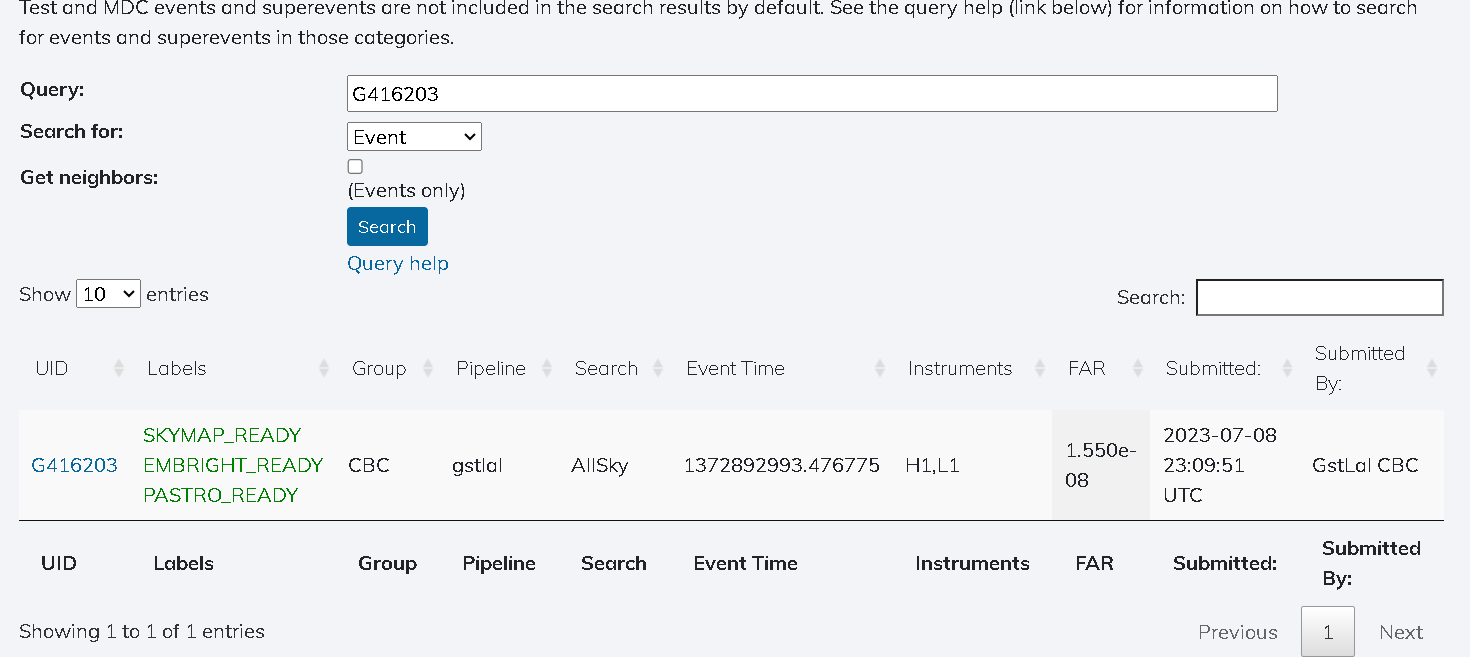
\includegraphics[width=0.6\textwidth]{figs/search.png}
\caption{Search G416203 at GraceDB}
\end{figure}

\subsubsection{See an Event}

Activate the environment. The environment name is that you have set.

\begin{verbatim}
    $ conda activate testlensing
\end{verbatim}

If you know the superevent ID(SID) or the event ID(GID), you can see the property of the (super)event.

\begin{verbatim}
    $ mkdir seeevent
    $ cd seeevent
    $ gracedb get event G416203
\end{verbatim}

\subsubsection{Set Up a TESLA Analysis}

This part is based on Doctor Alvin Li's TESLA guide, the part '\href{https://git.ligo.org/alvin.li/tesla#settting-up-a-tesla-analysis}{Setting up a TESLA analysis}'.

First, initialize the environment and login.

\begin{verbatim}
    $ conda actiavte testlensing
    $ htgettoken -a vault.ligo.org -i igwn
\end{verbatim}

Go to the home directory and make a directory to analyze.

\begin{verbatim}
    $ cd
    $ mkdir Projects
    $ cd Projects
    $ mkdir tesla_o4_runs
    $ cd tesla_o4_runs
    $ mkdir production
    $ cd production
\end{verbatim}

And set the environment.

\begin{verbatim}
    $ cp /home/lensing.o4/Projects/tesla_o4_runs/production/base_config.yml .
    $ ln -s /home/lensing.o4/Projects/tesla_o4_runs/production/S230518h
    $ ln -s /home/lensing.o4/Projects/tesla_o4_runs/production/S230529ay
    $ ln -s /home/lensing.o4/Projects/tesla_o4_runs/production/S230601bf
    $ ln -s /home/lensing.o4/Projects/tesla_o4_runs/production/S230605o
\end{verbatim}

Vim into the base-config file.

\begin{verbatim}
    $ vi base_config.yml
\end{verbatim}

And change those parts:

[basic\_information] -> project\_dir: (The project folder you analyze)

[basic\_information] -> x509\_proxy: ""

[general\_settings] -> group\_user: (your name, ex. albert.einstein)

[general\_settings] -> webdir: /home/(your name)/public\_html/(The folder which has same name as your project directory)

Please see inside the public\_html folder.

Start analysis.

\begin{verbatim}
    $ tesla_initiate_event_analysis --base-config base_config.yml --event G416203
\end{verbatim}

A master config file 'S230708cf\_TESLA-X\_version0\_main\_config.yml' will be generated under the directory 'S230708cf'.

Go to the directory and continue the analysis.

\begin{verbatim}
    $ cd S230708cf/
    $ tesla_initiate_event_analysis \
       --base-config S230708cf_TESLA-X_version0_main_config.yml
\end{verbatim}

If it seems to stop while executing the analysis, it will continue by pressing the Enter key. This case will happen many times.

You can watch the progress as follows in other sessions.

\begin{verbatim}
    $ cd (The project folder you analyze)/S230708cf/TESLA-X_version_0/injection_run/
    $ tail -f (FIX ME)
\end{verbatim}
